\section{Results}

\subsection{Creating a representative dataset of questions}
\label{creating_dataset}

We manually create a set of 4760 questions using the method explained in \cref{creating_dataset}.

In order to be able to reuse objects for different questions, we separated the questions and objects in 9 different categories.

\begin{enumerate}
	\item \textbf{Person} Historical people living from early antiquity to the present day from all around the globe. The questions have short, unambiguous answers, such as date of birth or most famous invention.
	\item \textbf{City} Cities from all over the globe. Questions may include population, founding date, notable landmarks, or geographical features.
	\item \textbf{Principle} Scientific principles, discovered from the 16th century forward. Questions about their discovery, use, and others.
	\item \textbf{Element} Elements from the periodic table. Questions may cover discovery, atomic number, chemical properties, or common uses.
	\item \textbf{Book} Literary works from various genres, time periods, and cultures. Questions may involve authors, publication dates, plot summaries, or literary significance.
	\item \textbf{Painting} Famous artworks from different art movements and periods. Questions may cover artists, creation dates, styles, or current locations.
	\item \textbf{Historical Event} Significant occurrences that shaped world history, from ancient times to the modern era. Questions may involve dates, key figures, causes, or consequences.
	\item \textbf{Building} Notable structures from around the world, including ancient monuments, modern skyscrapers, and architectural wonders. Questions may cover location, architect, construction date, or architectural style.
	\item \textbf{Composition} Musical works from various genres and time periods. Questions may involve composers, premiere dates, musical style, or cultural significance.
\end{enumerate}

Each one of these categories has a number of questions that are assigned one of the objects, enhancing the done by \citeauthor{factual_recall}.

The full list of base questions and objects for all categories can be found in \cref{appendixA}.
The total amount of these and composition of the 4760 questions can be found in \cref{category_amounts}.

\begin{table}[htb]
	\centering
	\scriptsize
	\begin{tabular}{>{\bfseries}l r r r}
		\toprule
			\bfseries Category & \bfseries Base Questions & \bfseries Objects & \bfseries Total Questions \\
		\midrule
			Person           &  17 &  57 &  969 \\
			City             &  17 &  70 & 1190 \\
			Principle        &   5 &  37 &  185 \\
			Element          &  15 &  43 &  645 \\
			Book             &  11 &  49 &  539 \\
			Painting         &  12 &  44 &  528 \\
			Historical Event &   4 &  64 &  256 \\
			Building         &   9 &  22 &  198 \\
			Composition      &  10 &  25 &  250 \\
		\midrule
			Total            & 100 & 411 & 4760 \\
		\bottomrule
	\end{tabular}
	\caption{The amount of base questions, objects, and the total amount of questions in each category on the final dataset.}
	\label{category_amounts}
\end{table}

\subsection{When does a model choose the provided context knowledge over its inherent knowledge?}

\subsubsection{Decoder-Only Models}

The results of running the experiment on the two Llama decoder-only models can be found in \cref{llama_table,llama_results}.

\begin{table}[htbp]
	\centering
	\footnotesize
	\begin{tabular}{l r r r}
		\toprule
			\bfseries Model & \bfseries Parametric & \bfseries Contextual & \bfseries Other \\
		\midrule
			\ttfamily llama-3.1-8B & 745 & 3662 & 353 \\
			\ttfamily llama-3.1-70B & 1070 & 3303 & 387 \\
		\bottomrule
	\end{tabular}
	\caption{Results when running all entries on a decoder-only model.}
	\label{llama_table}.
\end{table}

\begin{figure}[htbp]
	\centering
	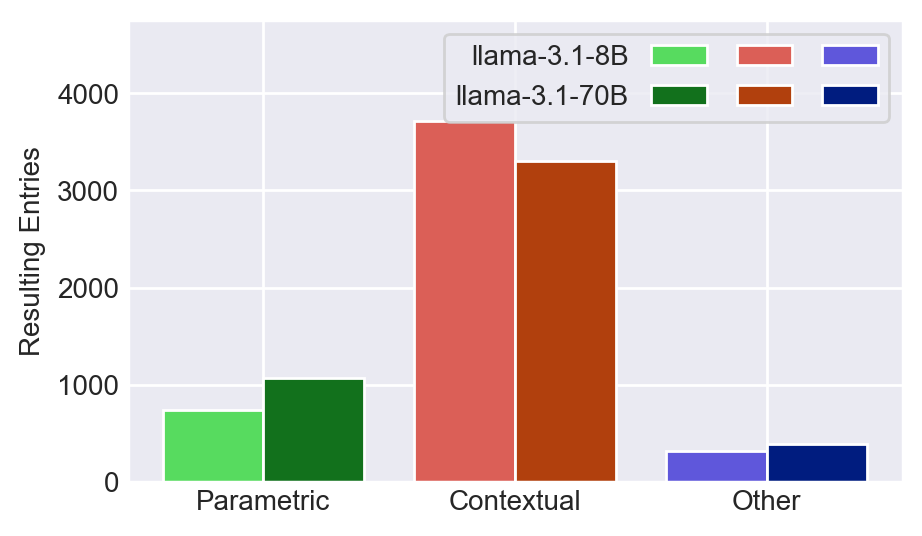
\includegraphics[width=.75\textwidth]{llama_amount.png}
	\caption{Resulting entries when running the queries from \cref{creating_dataset} with the Llama models}
	\label{llama_results}
\end{figure}

We can see from these results that larger models tend to get their answers from their parametric memory, even in the face of contradictory context.
This is further discussed in \cref{discussion}.

A similar pattern emerges in most (but not all) of the categories, which can be seen in \cref{llama_cats_table,llama_cats_result}.

\begin{table}[htbp]
	\centering
	\footnotesize
	\begin{tabular}{>{\bfseries}l | r r r | r r r}
		\toprule
			& \multicolumn{3}{c|}{\ttfamily \bfseries llama-3.1-8B} & \multicolumn{3}{c}{\ttfamily \bfseries llama-3.1-70B} \\
			& \bfseries Parametric & \bfseries Contextual & \bfseries Other & \bfseries Parametric & \bfseries Contextual & \bfseries Other \\
		\midrule
			Person           &  40 &  833 & 96 & 209 & 614 & 146 \\
			City             & 117 & 1007 & 66 & 166 & 966 &  58 \\
			Principle        &  44 &  118 & 23 &  44 & 117 &  24 \\
			Element          & 218 &  385 & 42 & 275 & 347 &  23 \\
			Book             & 135 &  344 & 60 & 154 & 318 &  67 \\
			Painting         &  47 &  458 & 23 &  49 & 445 &  34 \\
			Historical Event &  81 &  154 & 21 & 117 & 118 &  21 \\
			Building         &  27 &  163 &  8 &  31 & 159 &   8 \\
			Composition      &  36 &  200 & 14 &  25 & 219 &   6 \\
		\bottomrule
	\end{tabular}
	\caption{Results for running each one of the 10 categories separately on the Decoder-only models.}
	\label{llama_cats_table}
\end{table}

\begin{figure}[htbp]
	\centering
	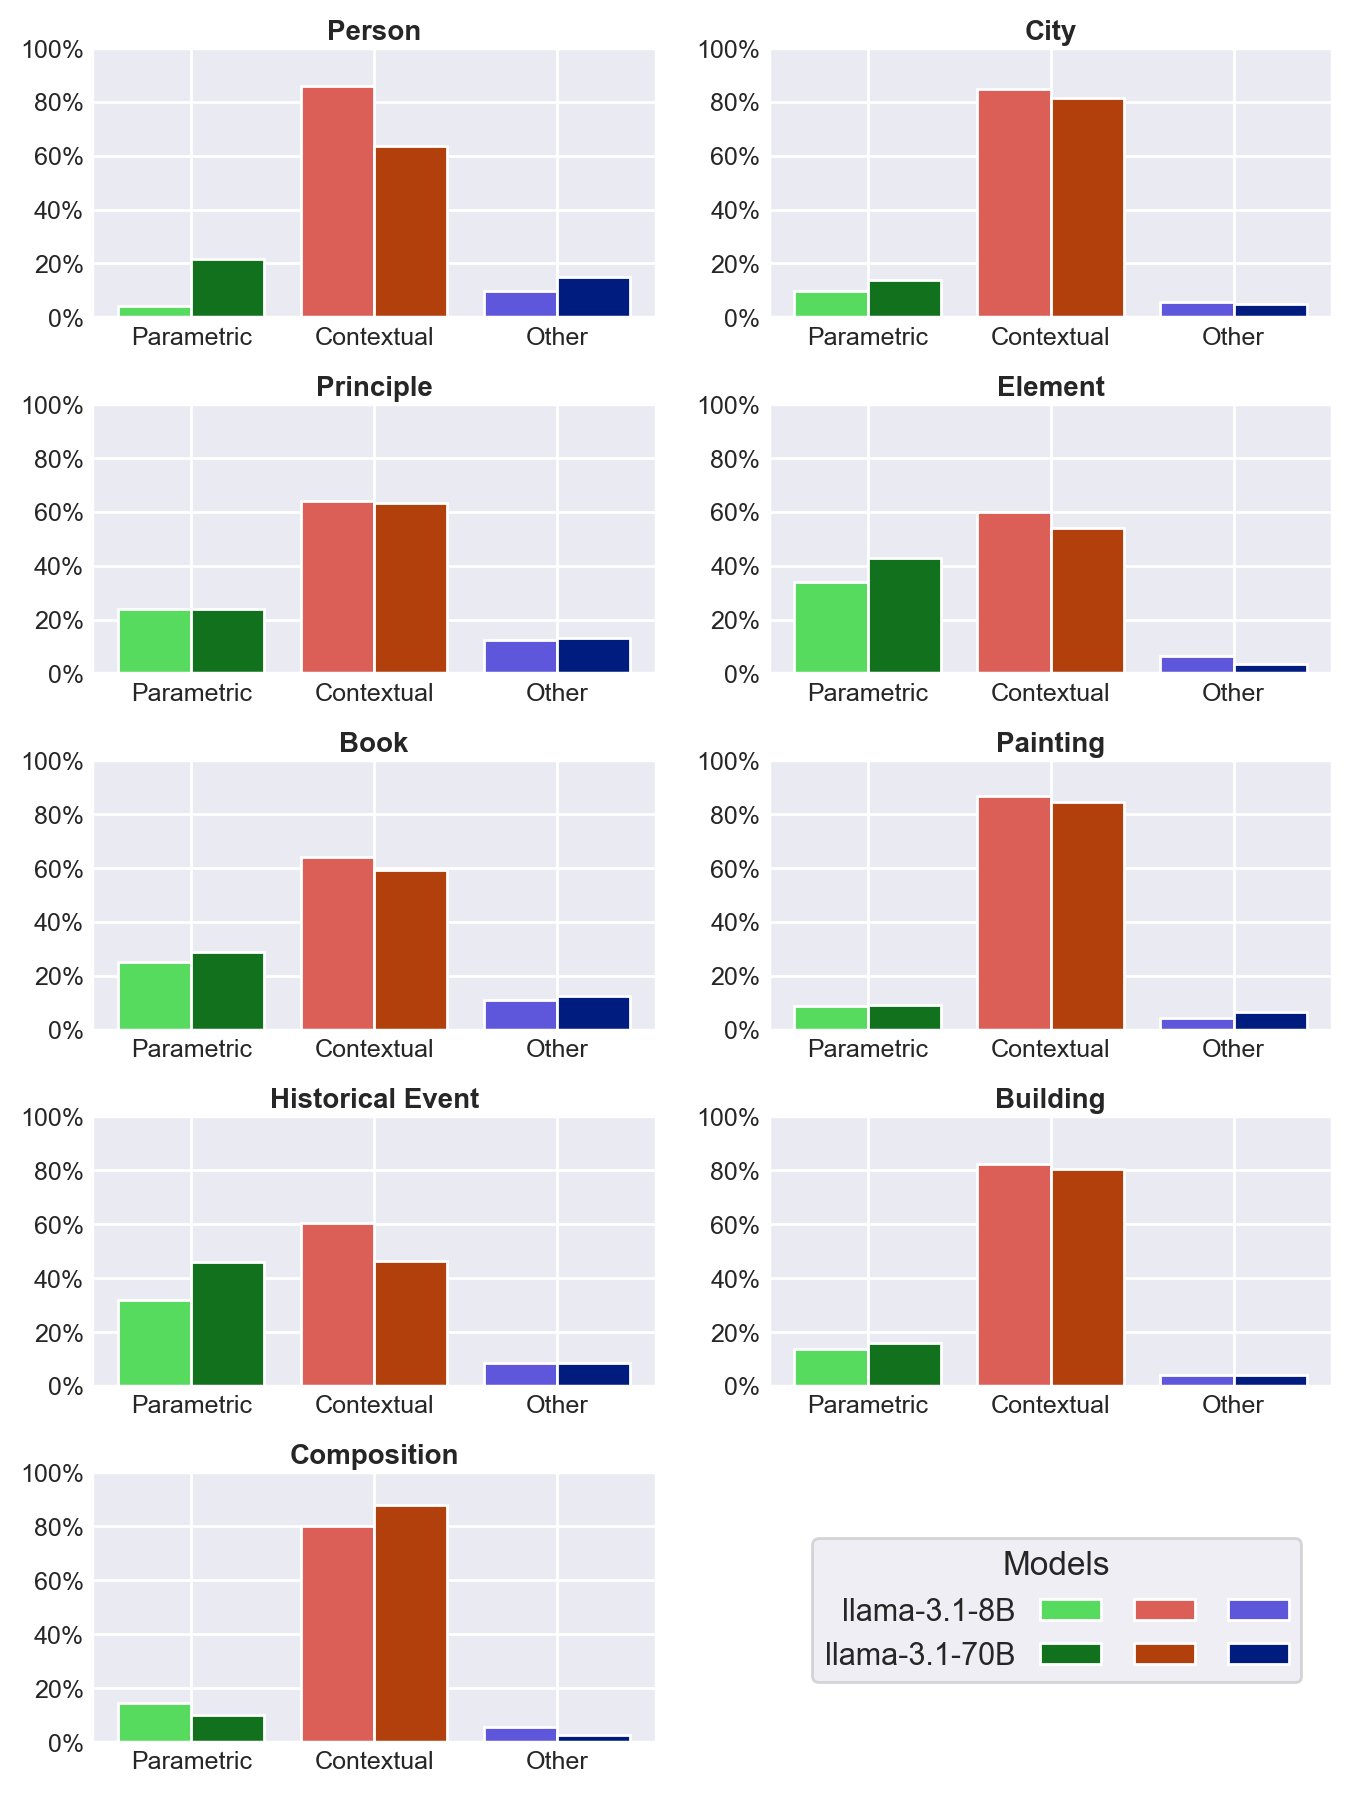
\includegraphics[width=\textwidth]{llama_allcats.png}
	\caption{Results of running decoder-only models on the queried data, grouped by category. This plots the information shown in \cref{llama_cats_table}.}
	\label{llama_cats_result}
\end{figure}

\subsubsection{Seq2Seq Models}

The results of running the experiments with the Seq2Seq Flan-T5 models can be found in \cref{flan_table,flan_results}.

\begin{table}[htbp]
	\centering
	\footnotesize
	\begin{tabular}{l r r r}
		\toprule
			& \bfseries Parametric & \bfseries Contextual & \bfseries Other \\
		\midrule
			\ttfamily flan-t5-xl  & 248 & 4284 & 228 \\
			\ttfamily flan-t5-xxl & 242 & 4304 & 214 \\
		\bottomrule
	\end{tabular}
	\caption{Results when running all entries on a Seq2Seq model.}
	\label{flan_table}
\end{table}

\begin{figure}[htpb]
	\centering
	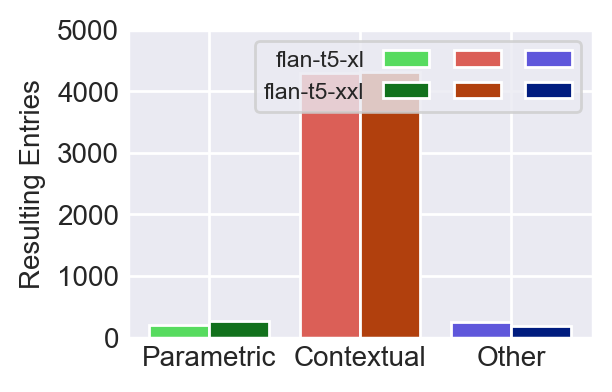
\includegraphics[width=.75\textwidth]{flan_amount.png}
	\caption{Resulting entries when running the queries from \cref{creating_dataset} with the Flan-T5 models.}
	\label{flan_results}
\end{figure}

Unlike the Decoder-only models, the results are almost identical between the small and large models.

The reason for this will be discussed later. \Cref{flan_cats_table,flan_cats_result} contain this information grouped by category.

\begin{table}[htpb]
	\centering
	\footnotesize
	\begin{tabular}{>{\bfseries}l | r r r | r r r}
		\toprule
			& \multicolumn{3}{|c}{\ttfamily flan-t5-xl} & \multicolumn{3}{|c}{\ttfamily flan-t5-xxl} \\
			& \bfseries Parametric & \bfseries Contextual & \bfseries Other & \bfseries Parametric & \bfseries Contextual & \bfseries Other \\
		\midrule
			Person           &  32 &  900 & 37 &  23 &  890 & 56 \\
			City             & 120 & 1030 & 40 &  78 & 1093 & 19 \\
			Principle        &  13 &  164 &  8 &   9 &  168 &  8 \\
			Element          &   6 &  637 &  2 & 102 &  515 & 28 \\
			Book             &  26 &  488 & 25 &  18 &  457 & 64 \\
			Painting         &  26 &  446 & 56 &   4 &  498 & 26 \\
			Historical Event &  11 &  217 & 28 &   1 &  254 &  1 \\
			Building         &  14 &  174 & 10 &   0 &  189 &  9 \\
			Composition      &   0 &  228 & 22 &   7 &  240 &  3 \\
		\bottomrule
	\end{tabular}
\end{table}
